\documentclass[11pt,a4paper]{article}

% ---------------------------------------------------------------------------
% Neuro3D: ResearchGate preprint (13 October 2026). Build:
%   pdflatex neuro3d_paper && bibtex neuro3d_paper && pdflatex neuro3d_paper && pdflatex neuro3d_paper
% ---------------------------------------------------------------------------
\usepackage[T1]{fontenc}
\usepackage[utf8]{inputenc}
\usepackage{lmodern}
\usepackage{amsmath,amssymb}
\usepackage[a4paper,top=2.5cm,bottom=2.6cm,left=2.5cm,right=2.5cm]{geometry}
\usepackage{microtype}
\usepackage{graphicx}
\usepackage{booktabs}
\usepackage{tabularx}
\usepackage{array}
\usepackage[font=small,labelfont=bf,labelsep=period,skip=5pt]{caption}
\usepackage{xcolor}
\usepackage{siunitx}
\usepackage[numbers,sort&compress]{natbib}
\usepackage{tikz}
\usetikzlibrary{arrows.meta,positioning,fit,calc}
\usepackage{enumitem}
\usepackage[colorlinks=true,linkcolor=blue!50!black,citecolor=blue!50!black,urlcolor=blue!50!black]{hyperref}

\sisetup{group-separator={,},group-minimum-digits=5,group-digits=integer,detect-all}
\setlist{itemsep=2pt,topsep=4pt}
\newtheorem{proposition}{Proposition}
\newcommand{\Emax}{E_{\max}}
\newcommand{\BU}{\,\mathrm{BU}}
\newcommand{\Fgeom}{F_{\mathrm{geom}}}
\newcommand{\Flin}{F_{\mathrm{lin}}}
\newcommand{\Fquad}{F_{\mathrm{quad}}}
\renewcommand{\arraystretch}{1.12}
\urlstyle{same}

\hypersetup{
  pdftitle={Coherent optical learning from 3D scene geometry with certified numerics},
  pdfauthor={Francisco Angulo de Lafuente},
  pdfsubject={Optical neural networks; certified numerics; reproducibility},
  pdfkeywords={coherent optics, optical neural networks, interval arithmetic, Lean, Blender, angular spectrum, reproducibility}
}

\title{\bfseries Coherent optical learning from 3D scene geometry with certified numerics: a prospective wave test, capacity limits and reproducible evidence}
\author{Francisco Angulo de Lafuente\\[2pt]
\small Independent researcher\\
\small Code and data: \url{https://github.com/Agnuxo1/Neuro3D}}
\date{\small Preprint, 13 October 2026. Not peer reviewed.}

\begin{document}
\maketitle

\begin{abstract}
\noindent
We ask whether an accessible 3D scene editor can serve as a reproducible instrument for a coherent optical classifier whose fields and trainable parameters come from evaluated scene geometry. A 104-object Blender scene is captured exactly and admitted as a 133-state graph covering \num{17060} terminal paths of an ideal scalar, monochromatic model. Sixteen mirror-pair translations are trained with geometry-derived gradients. On a previously examined Iris split the model reaches 27/30 held-out predictions, and 128-bit rational interval arithmetic certifies all 150 observed decisions (137 correct, 13 wrong). Wine comparisons show no advantage over matched baselines, and no end-to-end GPU cost advantage was observed. Lemmas T1--T5 behind the certificates are machine-checked in Lean~4. A prospective test with an independent mesh-free angular-spectrum solver confirms that a path model with free paraxial diffraction predicts Mach--Zehnder modal powers within $\Emax = 0.0040$ (budget 0.02) over 21 exact phases, whereas the model without diffraction fails ($\Emax = 0.0281$). The same criterion places every path of the captured scene far outside the diffraction-free regime ($\zeta$ from 47.7 to 225.7, against $\zeta \le 0.2857$): the represented ray model is a well-defined computational object, not a faithful wave description of that scene. The 16 translations span a 12-dimensional decision family, against 26 for a free linear optical class, and lose 0.051 test accuracy to it on synthetic linear-teacher tasks; a predicted benefit of quadratic capacity did not appear. A compiled operator is not faster when recompiled at every call. Protocols were committed before execution; negatives are retained.
\end{abstract}

\noindent\textbf{Keywords:} coherent optics; optical neural networks; interval arithmetic; formal verification; angular spectrum; differentiable geometry; reproducibility.

% ===========================================================================
\section{Introduction}
\label{sec:intro}

Optical hardware for machine learning is typically designed in specialised simulators, and the link between the geometry an engineer edits and the numbers a learning algorithm sees is not always auditable end to end. This work asks a narrower, operational question: can a widely available scene editor (Blender) serve as a reproducible instrument for an own coherent optical model, so that every field, gradient and decision can be traced to captured geometry and checked by independent numerical and formal means? We answer it for one represented model and one scene, and we report what this answer does \emph{not} establish.

The represented model is ideal, scalar, monochromatic and lossless planar optics in a homogeneous medium. It is not a calibrated photonic processor and not a solution of Maxwell's equations. A central result of this paper (Section~\ref{sec:wave}) is a prospective test that delimits the regime in which such a path model is a faithful wave description, and the finding that the captured scene, at its represented wavelength, lies far outside that regime.

\paragraph{Related work.}
Trainable coherent photonic networks and diffractive optical learning predate this work. Programmable Mach--Zehnder interferometer (MZI) meshes realise arbitrary unitary operators~\cite{reck1994,clements2016} and were used for coherent nanophotonic inference~\cite{shen2017}; diffractive deep networks learn with free-space propagation between passive layers~\cite{lin2018}; a coherent optical network learning phases from multiple optical path differences was reported earlier still~\cite{kawata2003}. Training on physical systems has been demonstrated with physics-aware training~\cite{wright2022} and with \emph{in situ} backpropagation on a photonic chip~\cite{pai2023}, both of which require calibrated physical measurements. Energy arguments for optical computing, including photoelectric multiplication~\cite{hamerly2019} and sub-photon-per-multiplication operation~\cite{wang2022}, concern physical devices; a GPU simulation does not inherit them. On the software side, scene-specific differentiable computation is mature: Dr.Jit compiles differentiable renderers~\cite{jakob2022}, differentiable non-sequential ray tracing optimises freeform optics~\cite{dekoning2023}, wave-optics models are combined with ray models for end-to-end imaging design~\cite{ho2024}, and coherent multipath geometry gradients appear in radio-frequency digital twins~\cite{chen2026}. Ray tracing on programmable graphics hardware~\cite{purcell2002}, GPU optical ray tracers with scene editors~\cite{mauch2013} and OptiX-based instrument models~\cite{keksel2023} rule out GPU optics as a contribution in itself, and interval and affine arithmetic have been used in ray tracing~\cite{knoll2009,moore2009}. These precedents bound what can be claimed here: neither optical learning, differentiable geometry, GPU optical tracing nor interval certification is new on its own.

\paragraph{Contributions.}
The candidate contribution is an integration with joint numerical certification, measured at its cost, and an honest characterisation of its limits:
\begin{enumerate}[label=(\roman*)]
  \item An exact capture of evaluated Blender geometry into a complete finite-state coherent graph, with every nonzero branch admitted or the computation declared incomplete (Section~\ref{sec:model}).
  \item Independent 128-bit rational enclosures of observed fields, powers and class decisions, conditional parameter-box certificates and an operator Gram certificate, with the arithmetic core of the certificate lemmas machine-checked in Lean~4 (Section~\ref{sec:cert}).
  \item Geometry-driven training with own derivatives, a native Blender save/reopen roundtrip and a full-cost GPU accounting with no observed end-to-end advantage (Section~\ref{sec:learn}).
  \item A prospective, preregistered wave confirmation (WAVE-C1) with an independent mesh-free solver, and the resulting regime map of the captured scene (Section~\ref{sec:wave}).
  \item A preregistered capacity test (HA-K1) showing that the captured geometry measurably restricts the free linear optical class, and a refuted speed prediction for a compiled operator (G1) (Sections~\ref{sec:capacity}--\ref{sec:g1}).
\end{enumerate}
We do not claim novelty proven against all prior art, superiority over classical baselines, a physical device, energy efficiency, external peer review or independent human replication.

\begin{figure}[t]
\centering
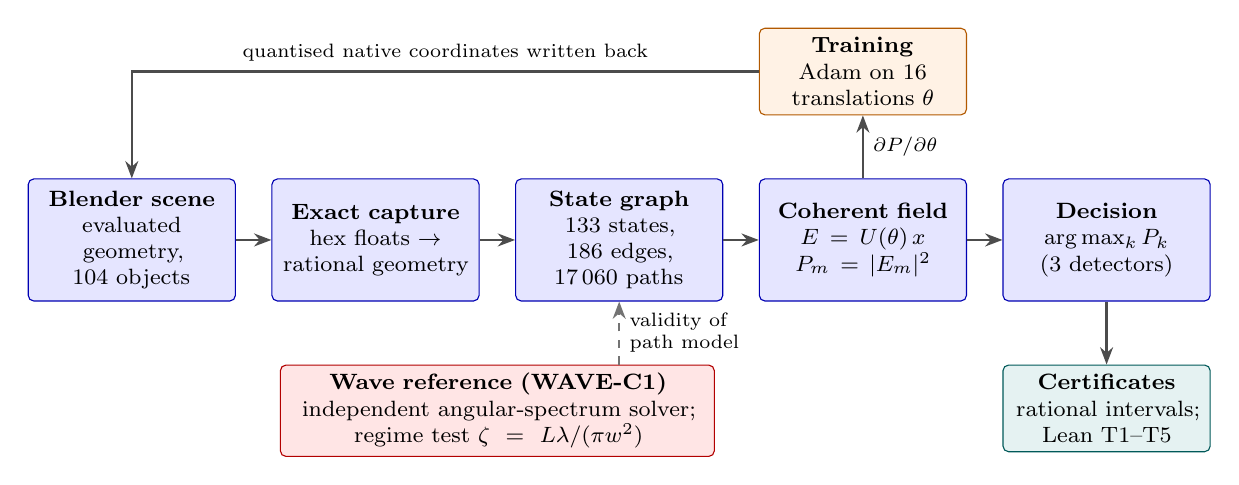
\begin{tikzpicture}[
  node distance=4mm and 4.5mm,
  box/.style={draw=#1!70!black, fill=#1!10, rounded corners=2pt, align=center,
              font=\footnotesize, text width=2.42cm, minimum height=1.55cm, inner sep=3pt},
  box/.default=blue,
  arr/.style={-{Stealth[length=2.2mm]}, thick, draw=black!70},
  darr/.style={-{Stealth[length=2.2mm]}, thick, dashed, draw=black!55}]
  \node[box] (scene) {\textbf{Blender scene}\\evaluated geometry,\\104 objects};
  \node[box, right=of scene] (cap) {\textbf{Exact capture}\\hex floats $\to$\\rational geometry};
  \node[box, right=of cap] (graph) {\textbf{State graph}\\133 states,\\186 edges,\\\num{17060} paths};
  \node[box, right=of graph] (field) {\textbf{Coherent field}\\$E = U(\theta)\,x$\\$P_m = |E_m|^2$};
  \node[box, right=of field] (dec) {\textbf{Decision}\\$\arg\max_k P_k$\\(3 detectors)};
  \node[box=orange, above=8mm of field, minimum height=1.1cm] (train) {\textbf{Training}\\Adam on 16 translations $\theta$};
  \node[box=teal, below=8mm of dec, minimum height=1.1cm] (cert) {\textbf{Certificates}\\rational intervals; Lean T1--T5};
  \node[box=red, anchor=north, text width=5.3cm, minimum height=1.1cm] (wave) at ($(cap.south)!0.5!(graph.south)+(0,-0.8)$) {\textbf{Wave reference (WAVE-C1)}\\independent angular-spectrum solver;\\regime test $\zeta = L\lambda/(\pi w^2)$};
  \draw[arr] (scene) -- (cap);
  \draw[arr] (cap) -- (graph);
  \draw[arr] (graph) -- (field);
  \draw[arr] (field) -- (dec);
  \draw[arr] (field) -- node[right,font=\scriptsize]{$\partial P/\partial\theta$} (train);
  \draw[arr] (train.west) -| node[pos=0.25,above,font=\scriptsize]{quantised native coordinates written back} (scene.north);
  \draw[arr] (dec) -- (cert);
  \draw[darr] (wave.north -| graph.south) -- node[right,font=\scriptsize,align=left]{validity of\\path model} (graph.south);
\end{tikzpicture}
\caption{Schematic of the pipeline (diagram only; contains no data). The scene is captured exactly, admitted as a complete finite-state graph and evaluated as a coherent linear map followed by quadratic detection. Training updates 16 mirror-pair translations that are written back to the scene as quantised native coordinates. Certificates enclose observed outputs and decisions; the separate wave reference tests in which regime the path model itself is valid.}
\label{fig:schematic}
\end{figure}

% ===========================================================================
\section{Model}
\label{sec:model}

\subsection{Scene ingress}
The capture reads Blender's evaluated dependency graph: mesh vertices, triangle indices, instance transforms, object identities, resolved source, parameter and detector bindings, and scene unit metadata. Floating-point values are stored in hexadecimal so that every exposed bit is preserved, and world geometry is rebuilt from them in rational arithmetic. This defines an exact affine \emph{represented} model; it does not certify the geometry an author intended, nor every rounding step of Blender's native transform pipeline. Coordinates and wavelength are in Blender units (BU); the represented wavelength is $\lambda = 0.1\BU$. Display scale is not a physical calibration, and reported powers are normalised scalar modal powers, not watts. Table~\ref{tab:scene} summarises the captured scene.

\begin{table}[t]
\centering
\caption{Captured scene and admitted graph (historical capture used throughout).}
\label{tab:scene}
\small
\begin{tabular}{@{}lr@{\hspace{2.2em}}lr@{}}
\toprule
Optical objects & 104 & Graph states & 133 \\
Triangles & \num{6656} & Graph edges & 186 \\
Coherent sources & 5 & Terminal path occurrences & \num{17060} \\
Terminal modes (3 class detectors) & 8 & Trainable mirror-pair translations & 16 \\
Coordinate bindings & 32 & Represented wavelength $\lambda$ & $0.1\BU$ \\
\bottomrule
\end{tabular}
\end{table}

\subsection{Coherent scalar model and detector semantics}
Inputs are explicit complex amplitudes $x \in \mathbb{C}^5$ with a common launch-phase reference. The temporal convention is $e^{-i\omega t}$, so a segment of optical length $L$ contributes $e^{+i 2\pi L/\lambda}$; mirrors and splitters carry declared phase and sign conventions. For a terminal mode $m$ the field is the coherent sum over its admitted paths,
\begin{equation}
  E_m(\theta) = \sum_{p \in \mathcal{P}_m} \Big(\prod_{e \in p} c_e\Big)\, e^{\,i 2\pi L_p(\theta)/\lambda}\; x_{s(p)},
  \qquad P_m = |E_m|^2,
  \label{eq:field}
\end{equation}
where $c_e$ are the local reflection or transmission coefficients, $L_p$ the geometric path length and $s(p)$ the source of path $p$. At fixed geometry $E = U(\theta)\,x$ with $U \in \mathbb{C}^{8\times5}$. Summing intensities of independently labelled sources instead would remove interference cross terms and define a different classifier. Three fixed detectors $k \in \{0,1,2\}$ carry the class decision. An estimated $\arg\max_k P_k$ is \emph{not} automatically certified: a decision is certified only when the lower bound of the winning power exceeds the upper bound of every competitor; zero input and overlapping bounds remain \emph{unknown}.

\subsection{Complete finite-state propagation}
A state identifies a represented origin, direction and previous optical plane. Two states merge only when these quantities are exactly identical, so that their future propagation operators coincide. Every nonzero transmission or reflection remains an edge, and only mathematically exact zero coefficients omit one. Cycles, unresolved intersections, missing support or exhausted resources produce an \emph{incomplete} status, never a fabricated field. A conservative object-level bounding-box index narrows candidate work without changing the closed triangle predicates, and coincident triangle edges are checked by an independent interior witness so that shared vertices do not create artificial optical edges. The captured graph has 133 states and 186 edges and preserves all \num{17060} terminal path occurrences. It represents the admitted scalar network, not the set of physical paths of any real device.

\subsection{Geometry-driven derivatives and training}
For fixed plane normals and admitted paired translations $\theta \in \mathbb{R}^{16}$, ray--plane intersections give exact affine derivatives of origins, hits and segment lengths; a merge is admitted only when the incoming affine origin derivatives agree. Field derivatives propagate through every edge, and power derivatives follow from $\partial P_m/\partial\theta_j = 2\,\mathrm{Re}\big(\overline{E_m}\,\partial E_m/\partial\theta_j\big)$. No historical analytic weight matrix supplies fields or gradients. Training minimises the cross entropy of $\mathrm{softmax}(P_k/T)$ with a fixed temperature $T = 0.05$, using Adam on the 16 world-$x$ translations. Proposed positions are quantised to Blender's float32 coordinates within a declared box (centre $\pm 0.035\BU$), every evaluated optimizer state is independently audited, and a fresh final geometric rebuild checks the affine computation. Finite differences and an autograd reference are software controls, not universal gradient certificates.

\subsection{Rank limits of passive coherent detection}
\begin{proposition}\label{prop:rank}
Let detector $k$ have field row $a_k + i b_k$ with $a_k, b_k \in \mathbb{R}^5$. For real input $x \in \mathbb{R}^5$, $P_k = x^{\top} Q_k x$ with $Q_k = a_k a_k^{\top} + b_k b_k^{\top}$, which is positive semidefinite of rank at most two; the difference of two detector powers is a quadratic form of rank at most four. For complex input, $P_k = x^{\dagger} u_k u_k^{\dagger} x$ with a Hermitian form of rank at most one.
\end{proposition}
The proof is immediate from $P_k = (a_k^{\top}x)^2 + (b_k^{\top}x)^2$. These restrictions are algebraic, not a numerical-threshold observation. The model has no intermediate optical nonlinearity and does not claim universal approximation; the only nonlinearity is quadratic detection, followed by the argmax. Normalising the common input power is part of the declared encoding and is shared with all classical comparisons.

% ===========================================================================
\section{Certified numerics}
\label{sec:cert}

\subsection{Exact graph admission}
An independent auditor, separate from the producer, recomputes nearest hits and branch admissibility in exact rational arithmetic. Completeness, geometric correctness, enclosure correctness and classification accuracy are distinct acceptance conditions. The certificate claim is falsifiable: one independently verified exact represented-model output outside a claimed enclosure, one invalid certified decision, or one unbounded omitted nonzero branch refutes it.

\subsection{Interval enclosures of observed outputs}
Enclosures use rational outward rounding at 128 bits, an interval for $\pi$ from Machin's series with a remainder bound, square-root bounds from integer arithmetic and exact rational Taylor evaluation with explicit remainders~\cite{moore2009}; complex sums and powers are composed through the audited graph. They bound an already observed native output against the exact represented model; they do not claim that every libm or GPU execution has the same error. The first enclosure was valid but too loose (field $L_1$ bound \num{1.51e-7}, power bound \num{1.93e-7}, both above the fixed $10^{-11}$ budgets); it is archived. A revised exact-midpoint Taylor composition, published before its recomputation with unchanged budgets, gives the bounds in Table~\ref{tab:cert}, and an independently written 90-digit composition fell inside every reported interval.

\begin{table}[t]
\centering
\caption{Certificates of observed outputs against the exact represented model. Budgets were fixed before computation ($10^{-11}$ for fields and powers unless stated). ``Ideal'' refers to the train-only feature encoding computed from parsed binary64 values.}
\label{tab:cert}
\footnotesize
\begin{tabularx}{\textwidth}{@{}>{\raggedright\arraybackslash}p{3.45cm}ll>{\raggedright\arraybackslash}X@{}}
\toprule
Object (inputs) & Field $L_1$ bound & Power bound & Decisions \\
\midrule
Represented graph (unit input) & \num{4.9383434427813286e-15} & \num{3.1372973883238074e-15} & R1 lower margin \num{0.18933601504039158} \\
Trained native graph, CPU (150 Iris rows, ideal encoding) & \num{2.7683e-15} & \num{1.0366e-15} & 150 separated: 137 correct, 13 wrong; margin $\ge$ \num{2.11197e-4} \\
CUDA complex128 evaluation (60 probes) & \num{2.9356883e-15} & \num{1.3807709e-15} & 59 certified; zero input unknown \\
Final native graphics scene, shader + CPU merge (150 rows; recorded / ideal inputs) & \begin{tabular}[t]{@{}l@{}}\num{9.97351e-14}\\ \num{9.97449e-14}\end{tabular} & \begin{tabular}[t]{@{}l@{}}\num{7.15061e-15}\\ \num{7.09172e-15}\end{tabular} & 150 separated, 0 unknown; 137 correct, 13 wrong \\
\midrule
Parameter boxes $\times1$, $\times10$, $\times100$, $\times1000$ (150 rows) & \multicolumn{2}{l}{topology proved for all four boxes} & 147, 131, 40, 0 decisions preserved; rest unknown \\
Operator Gram $U^{\dagger}U$ (all $x \in \mathbb{C}^5$) & \multicolumn{2}{l}{$\big|\|Ux\|^2-\|x\|^2\big| \le \varepsilon\|x\|^2$} & rank 5; $\varepsilon \le \num{3.0665868333669135e-19}$ \\
\bottomrule
\end{tabularx}
\end{table}

\subsection{Decision certificates and conditional robustness}
Numerical separation is not class correctness: of the 150 certified Iris decisions of the trained native graph, 137 are correct and 13 wrong, with minimum lower margin \num{2.11197e-4}. A separately frozen study defines 16 paired-translation boxes from the half-spacing of adjacent binary32 coordinates and expands them by factors 1, 10, 100 and 1000. Exact affine plane expressions prove the surface support and exclude all \num{13699} competitor-object opportunities across the 133 states for every box; interval coherent fields then preserve 147, 131, 40 and 0 of 150 argmax decisions, respectively. Remaining decisions are \emph{unknown}, not shown to be unstable. These are conditional represented perturbations, not manufacturing tolerances. A whole-family certificate proves all 133 state topologies over the original training box ($\pm0.035\BU$ plus quantisation allowance) in \SI{71.968}{s}. For the final operator, Hermitian interval $LDL^{\top}$ certifies column rank five and Gershgorin bounds place every eigenvalue of $U^{\dagger}U$ in $[1-\varepsilon, 1+\varepsilon]$, an approximate isometry over all eight terminal modes, of which the three class detectors are a subset (\SI{6.468}{s}, \SI{46.207}{MiB}).

\subsection{Machine-checked lemmas}
The certificates rest on five elementary lemmas (Table~\ref{tab:lean}). T1 was compiled earlier for any order satisfying two mixed transitivity requirements. T2--T5 are proved in core Lean~4.34~\cite{demoura2021} without Mathlib, over the integers; \texttt{\#print axioms} lists only \texttt{propext}, \texttt{Classical.choice} and \texttt{Quot.sound}, there is no \texttt{sorry}, and an external Linux continuous-integration job recompiles all five. Because the statements are over $\mathbb{Z}$, their use for rationals is by scaling with a common positive denominator. An independent red-team agent showed that the T3 hypotheses force an eventually zero integer sequence; the rational use of T3 is therefore per fixed partial tail $(K, m)$, by truncation, scaling and zero extension. Real and complex instantiations, the operator-norm link for T3, infinite sums and the rank-four bound for a detector difference remain open. The lemmas certify the arithmetic core of the certificates, not that any producer's numbers satisfy their hypotheses.

\begin{table}[t]
\centering
\caption{Certificate lemmas and their formal status (source \texttt{Lean/closure-core}).}
\label{tab:lean}
\small
\begin{tabularx}{\textwidth}{@{}l>{\raggedright\arraybackslash}p{3.3cm}>{\raggedright\arraybackslash}X@{}}
\toprule
Lemma & Lean name & Statement (informal) \\
\midrule
T1 & \texttt{separatedBoxes} & If $\ell_i \le P_i \le u_i$ for all $i$ and $u_i < \ell_w$ for every $i \ne w$, then $P_i < P_w$ for every $i \ne w$. \\
T2 & \texttt{powerPerturbation} & For $|E_{\mathrm{obs}}| \le A$ and $|E_{\mathrm{true}} - E_{\mathrm{obs}}| \le e$: $\big|\,|E_{\mathrm{true}}|^2 - |E_{\mathrm{obs}}|^2\big| \le 2Ae + e^2$. \\
T3 & \texttt{neumannTail} & If $n_k \ge 0$ and $q\,n_{k+1} \le p\,n_k$ with $0 \le p < q$, then $(q-p)\,q^{K+1}\sum_{k=K+1}^{K+m} n_k \le q\,p^{K+1} n_0$ (scaled partial tail). \\
T4 & \texttt{detectorRankTwo}, \texttt{hermitianRankOne} & Every $3\times3$ minor of $aa^{\top}+bb^{\top}$ vanishes (rank $\le 2$); principal $2\times2$ minors of the complex Gram form vanish. \\
T5 & \texttt{splitterPassive} & A two-port with $|t|^2+|r|^2 \le 1$ and $\mathrm{Re}(t\bar r)=0$ does not increase total output power. \\
\bottomrule
\end{tabularx}
\end{table}

% ===========================================================================
\section{Learning from geometry}
\label{sec:learn}

\subsection{Iris: a historical result with its limits}
The declared Iris split~\cite{fisher1936,uciiris} has 120 training and 30 held-out examples. Training-only min/max preprocessing maps the four features to four coherent sources plus a fixed coherent reference, with joint unit input power and no held-out clipping. Iris had been examined earlier in the project, so this is not a blind discovery. Historical learned delays were reset to an explicit untrained absolute geometry. Sixty fixed Adam updates reduced the training loss from \num{6.2554405} to \num{0.3097067}; training accuracy was 110/120 and held-out accuracy 27/30. All 61 represented states passed their geometry audits; the largest initial finite-difference gradient discrepancy was \num{1.4746713e-6} (tolerance $10^{-4}$) and the fresh-geometry field reconstruction differed by at most \num{4.6194484e-16}.

\subsection{Native Blender roundtrip and graphical learning}
Blender 4.5.14 applied the final native coordinates, saved a new file, reopened it with script execution disabled, recaptured the geometry and rebuilt the inference graph: all 150 observed powers had maximum difference zero and all predictions matched, with the original file unchanged. This is a bounded local roundtrip, not external replication. A separate, prospectively published protocol then performed the complete learning loop through native graphics: each of the 61 optimizer states was applied to the actual scene and recaptured, OpenGL raster/depth selected surfaces, and FP64 fragment shaders derived distances, phases and optical tangents; topology admission and compensated coherent merging remained on the CPU. Loss decreased from \num{6.25544053835} to \num{0.309706672112}, with 110/120 training and 27/30 held-out accuracy, and the quantised positions matched the CPU reference optimizer exactly. Across states the largest differences from the CPU reference were \num{8.99309e-14} (field) and \num{1.03455e-11} (loss gradient). The whole supervised run took \SI{3066.598253}{s}, of which \SI{2692.497419}{s} were graphical transports and CPU merges. The final scene is certified in Table~\ref{tab:cert}.

\subsection{Prospectively fixed Wine comparison}
Wine~\cite{uciwine} (178 examples) was used with four features fixed before training (alcohol, malic acid, ash, alkalinity of ash), one stratified 141/37 split and three fixed initialisation seeds. Linear softmax (15 coefficients) and quadratic softmax (45 coefficients) used the same encoding, split and labels. Table~\ref{tab:wine} shows the outcome. The three geometric runs share the same 37 held-out observations and cannot be pooled; paired exact McNemar~\cite{mcnemar1947} $p$-values against either baseline were 1, 0.5 and 0.125, uncorrected. No optical superiority is shown, and the spread across seeds indicates sensitivity to initialisation.

\begin{table}[t]
\centering
\caption{Prospectively fixed Wine comparison (one split, 37 held-out examples; Wilson~\cite{wilson1927} 95\,\% intervals).}
\label{tab:wine}
\small
\begin{tabular}{@{}lccc@{}}
\toprule
Model & Training correct & Held-out correct & Held-out 95\,\% interval \\
\midrule
Geometric, seed 1049 & 117/141 & 33/37 & 75.3--95.7\,\% \\
Geometric, seed 1050 & 108/141 & 30/37 & 65.8--90.5\,\% \\
Geometric, seed 1051 & 105/141 & 28/37 & 59.9--86.6\,\% \\
Linear softmax & 120/141 & 32/37 & 72.0--94.1\,\% \\
Quadratic softmax & 121/141 & 32/37 & 72.0--94.1\,\% \\
Training majority & 56/141 & 15/37 & 26.3--56.5\,\% \\
\bottomrule
\end{tabular}
\end{table}

\subsection{GPU cost: a retained negative}
All GPU measurements used one NVIDIA RTX~3090 admitted through a shared queue; AMD hardware was not available. Table~\ref{tab:cost} collects paired measurements at equal outputs. Warm CUDA evaluation of the cached graph (fields, powers and Jacobians in complex128, with geometry prepared on the CPU) was faster than the CPU only at batch 2048; every full-cost pair, including complete training, graph construction and native-graphics inference, was slower on the GPU. The first full graphical training attempt was stopped after its first state took \SI{322.45}{s}; a later equal-output comparison on identical geometry found deferred shading slower than forward shading (\SI{42.973787}{s} versus \SI{38.272944}{s}), so the historical observation cannot show that deferred shading accelerated learning. An earlier ratio of about 2.85 between two construction routes was traced, by an alternating ablation with identical exact refinement, to the algorithm rather than to the GPU (median CPU/GPU ratio 0.99034). Whole-GPU power samples include display activity and do not isolate kernel energy (Figure~\ref{fig:cost}).

\begin{table}[t]
\centering
\caption{Paired CPU/GPU measurements with identical outputs (wall-clock seconds unless stated; single shared host, no timing confidence intervals). Warm rows are synchronised medians of five repetitions and exclude preparation and transfers.}
\label{tab:cost}
\footnotesize
\begin{tabular}{@{}lrr@{}}
\toprule
Comparison & CPU route & GPU route \\
\midrule
Full Iris training, 60 updates (CUDA arithmetic) & 370.46 & 390.09 \\
Graph construction, identical refinement (3 pairs) & 9.83--9.90 & 9.91--10.00 \\
Warm cached-graph evaluation, batch 1 (ms) & 14.45 & 24.50 \\
Warm cached-graph evaluation, batch 2048 (ms) & 75.00 & 25.72 \\
Graph reconstruction: CPU BVH vs Cycles OptiX & 10.330787 & 41.008216 \\
Native inference, batch 1 (first / second) & 0.026788 / 0.020904 & 0.592882 / 0.335261 \\
Native inference, batch 150 (first / second) & 0.020160 / 0.031941 & 4.027876 / 3.458444 \\
Native inference, batch 4096 (first / second) & 0.024342 / 0.026418 & 98.006908 / 97.720299 \\
\bottomrule
\end{tabular}
\end{table}

\begin{figure}[t]
\centering
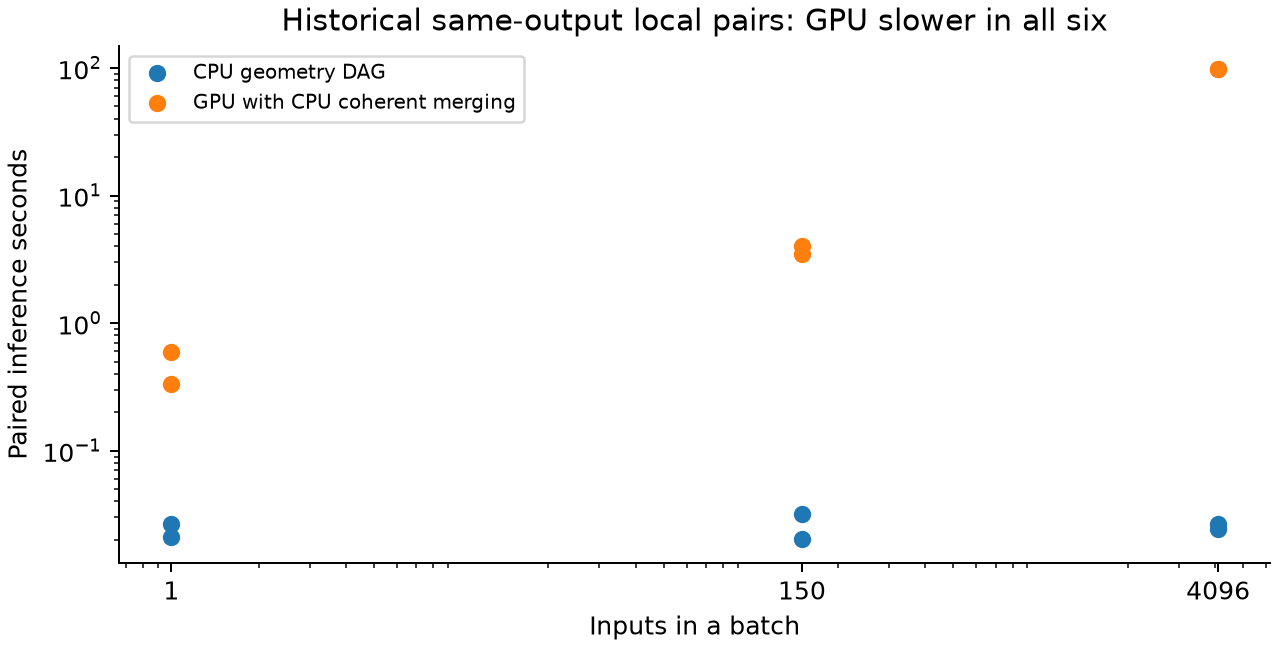
\includegraphics[width=0.6\textwidth]{figures/paired-cost.png}
\caption{Historical same-output inference pairs for batches of 1, 150 and 4096 inputs (log scale). The GPU route (FP64 shaders with CPU coherent merging) is slower in all six pairs; setup and proof costs are recorded separately in the protocols. These are descriptive local measurements, not energy or photonic-device results.}
\label{fig:cost}
\end{figure}

% ===========================================================================
\section{Prospective wave confirmation (WAVE-C1)}
\label{sec:wave}

\subsection{Background: a retained negative}
An earlier preregistered two-dimensional finite-difference time-domain (FDTD) test of a single MZI (P1-7) refuted the scalar path model without diffraction: maximum absolute modal-power errors were \num{0.0269264} at mesh $\lambda/16$ and \num{0.0275190} at $\lambda/24$, above the unchanged 0.02 budget (Figure~\ref{fig:wavenegative}). An exploratory Gaussian diffraction correction gave \num{0.0051349} and \num{0.0046153}, but that test used 12 and 18 discrete phases, per-mesh recalibrated film indices and an explanation found after the fact. WAVE-C1 tested the explanation prospectively.

\begin{figure}[t]
\centering
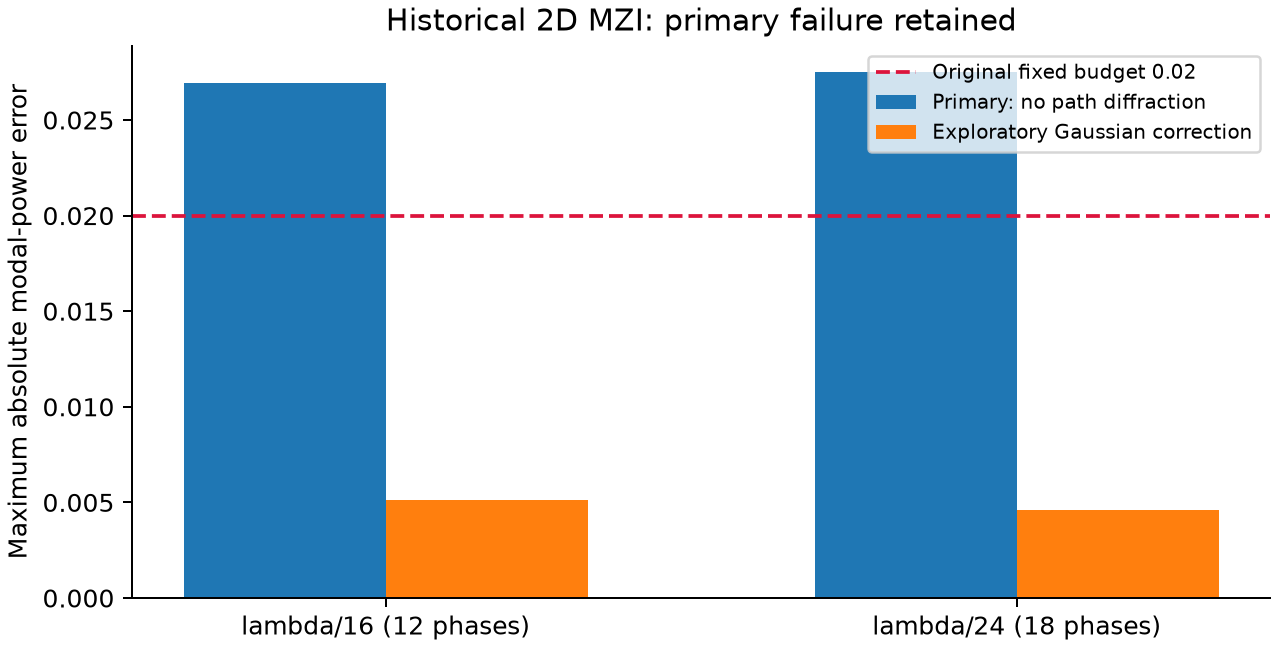
\includegraphics[width=0.56\textwidth]{figures/wave-negative.png}
\caption{Historical 2D MZI test (P1-7). The preregistered path model without diffraction misses the fixed 0.02 budget at both meshes; the exploratory Gaussian correction is shown for context only and motivated the prospective test of Section~\ref{sec:wave}. This is not a validation of the full network.}
\label{fig:wavenegative}
\end{figure}

\subsection{Solver, device and preregistered hypotheses}
The reference is a new mesh-free angular-spectrum solver that shares no code with the FDTD: 2D scalar $E_z$ (s-polarisation at the film), exact plane-wave (angular-spectrum) propagation, without the band-limited sampling variant of~\cite{matsushima2009}, exact Airy coefficients of a lossless slab and perfect-conductor mirrors, applied to infinite planar elements in the declared order. Its only idealisation beyond the 2D scalar model is the absence of element truncation and edge diffraction. Because no mesh represents the device, the \emph{same continuous device} is used at every numerical resolution: a slab of index $n = 2.537430764948469$ and thickness $d = \lambda/4$, the project's analytic 50/50 design at $45^\circ$. Mirror displacement realises all 21 phases exactly (effective path difference $j\lambda/20$, $j = 0,\dots,20$). The input is an exact Helmholtz beam of waist $w = 8\lambda$, propagating about $95\lambda$. The models under test are the frozen P1-7 path formula without (M0) and with (M1) free paraxial Gaussian diffraction in one transverse dimension, using the device's own central-angle coefficients and no fitted parameter. The error statistic is $\Emax = \max_{j,\text{port}} |P_{\text{solver}} - P_{\text{model}}|$ over 21 phases and two ports. The protocol was committed and pushed (commit \texttt{7327b67}; GitHub activity 2026-10-12T21:43:23Z) before the single run started at 21:43:30Z. Because the exploratory values were known and stated as predictions (about 0.005 for M1 and 0.027 for M0), the test is a confirmation, \emph{not} a blind test.

\subsection{Results}
Table~\ref{tab:wave} lists the decisions and Figure~\ref{fig:wave} the full sweep. The solver was self-consistent to \num{2.7e-15} across spectral sampling and window variants and conserved energy to \num{3.3e-16}, so both model decisions are valid. M1 stayed within $\Emax = \num{0.00401}$ of the reference: \emph{confirmed} in the declared regime. M0 erred by \num{0.02813}, \emph{replicating} the P1-7 refutation. The run took \SI{5.8}{s} of CPU on one thread, and an external Linux job with different Python, NumPy and SciPy versions reproduced every power within \num{8.9e-16}.

\begin{table}[t]
\centering
\caption{WAVE-C1 preregistered decisions (single execution, 12 October 2026).}
\label{tab:wave}
\small
\begin{tabularx}{\textwidth}{@{}>{\raggedright\arraybackslash}X>{\raggedright\arraybackslash}p{4.4cm}lc@{}}
\toprule
Hypothesis & Statistic & Budget & Result \\
\midrule
Solver self-consistency (3 variants vs reference) & $\max|\Delta P| = \num{2.7e-15}$ & $\le 10^{-9}$ & met \\
Energy balance, all phases and variants & $\max|\Phi_{\text{out}}/\Phi_{\text{in}}-1| = \num{3.3e-16}$ & $\le 10^{-9}$ & met \\
H-C1: M1, free paraxial diffraction & $\Emax = \mathbf{0.00401}$ & $\le 0.02$ & \textbf{confirmed} \\
H-C0: M0, no diffraction (P1-7 model) & $\Emax = \mathbf{0.02813}$ & $> 0.02$ & \textbf{replicated} \\
H-C2: archived FDTD vs reference with FDTD-calibrated splitter & $\max|\Delta P| = 0.00482$ ($\lambda/16$), $0.00456$ ($\lambda/24$) & $\le 0.005$ & supported \\
H-C3: two-MZI cascade, M1 & $\Emax = 0.00441$ (M0: 0.1066) & $\le 0.02$ & confirmed \\
\bottomrule
\end{tabularx}
\end{table}

\begin{figure}[t]
\centering
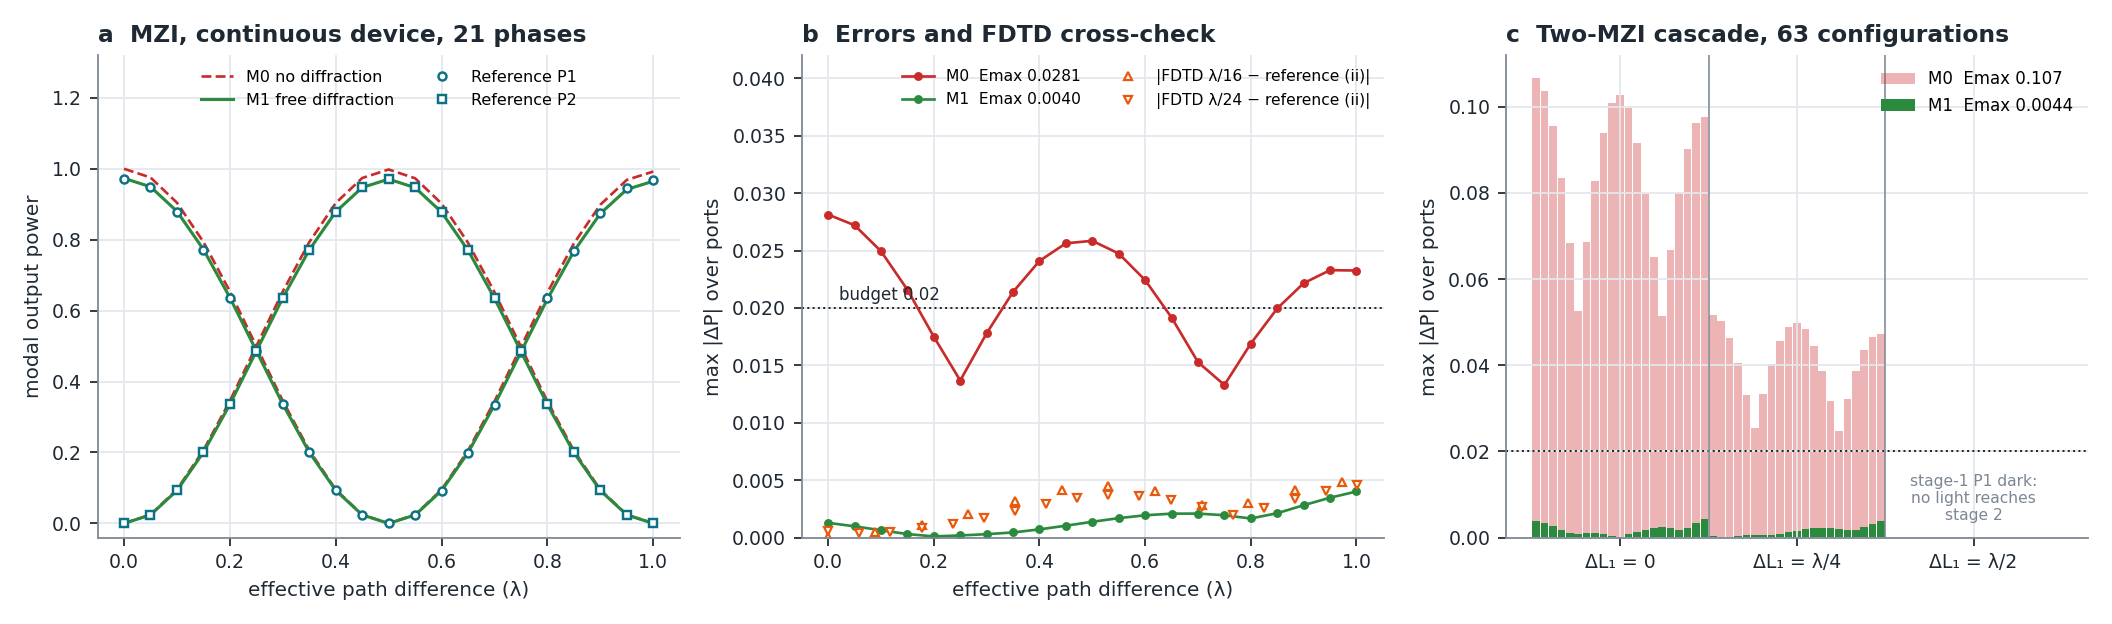
\includegraphics[width=\textwidth]{figures/wave-c1-confirmation.png}
\caption{WAVE-C1 with the same continuous device at every resolution. (a) Modal output powers of the reference solver (markers) and of the path models M0 (dashed) and M1 (solid) over 21 exact phases. (b) Maximum error over ports: M0 exceeds the 0.02 budget at most phases, M1 stays below 0.0041; triangles show the archived FDTD powers against the reference with the FDTD-calibrated splitter. (c) Two-MZI cascade over 63 configurations; the 21 configurations with stage-1 path difference $\lambda/2$ carry no light into stage 2 and test nothing.}
\label{fig:wave}
\end{figure}

\paragraph{FDTD cross-check.} The archived FDTD powers agree with an exact free-space propagation through an ideal splitter carrying the FDTD-calibrated coefficients within 0.0048, a narrow margin to the 0.005 budget. The FDTD transfer is therefore explained by free diffraction plus its splitter coefficients. With the same refractive index the agreement disappears (0.098 at $\lambda/16$, 0.020 at $\lambda/24$): the discrete FDTD films behave as different continuous devices, as their per-mesh calibrated indices already indicated. The continuous 50/50 slab agrees better than the ideal splitter (0.0033 and 0.0023).

\paragraph{Cascade.} Two cascaded MZIs with about $190\lambda$ of propagation keep M1 within 0.0044, while M0 errs by up to 0.107. A design weakness found after execution is retained: with stage-1 path difference $\lambda/2$ all light leaves stage 1 by the other port, so 21 of the 63 configurations carry no light into stage 2. The decision is unchanged on the 42 informative configurations. The cascade is solved sequentially with infinite planes; it confirms the path law along the unfolded cascade, not a full-geometry wave simulation.

\subsection{The captured network is outside this regime}
For a circular Gaussian beam of waist $w$ propagating a distance $L$ without refocusing, the power coupled back into the launch mode is $(1+\zeta^2/4)^{-1}$ with
\begin{equation}
  \zeta = \frac{L\lambda}{\pi w^2},
  \label{eq:zeta}
\end{equation}
that is, $L$ in units of the Rayleigh range $\pi w^2/\lambda$~\cite{kogelnik1966}; the 2D law tested above is its one-dimensional factor $(1+\zeta^2/4)^{-1/2}$. The declared criteria (no-diffraction power error $\le 0.02$, hence $\zeta \le 0.2857$; clipping $\le 10^{-3}$ per axis, hence half-aperture $\ge 1.645\,w$) were applied to every terminal path of the captured scene (Table~\ref{tab:regime}, Figure~\ref{fig:regime}). Every element is a $4\lambda$ square (detectors $3\lambda$), giving a projected aperture of $2.83\lambda$ at $45^\circ$, while paths are $110.7\lambda$ to $523.9\lambda$ long. With the largest unclipped beam, $\zeta$ ranges from 47.7 to 225.7. \textbf{No path (0 of \num{17060}) is in regime at $\lambda = 0.1\BU$}; all would need $\lambda \le \num{1.27e-4}\BU$, about 790 times shorter, or apertures about 28 times wider relative to the paths. The largest admissible waist ($0.86\lambda$) is itself not paraxial, so the criterion errs in the direction that favours this conclusion. The 3D criterion is the separable extension of the tested 2D law and remains a modelling statement.

\begin{table}[t]
\centering
\caption{Diffraction regime of the captured network ($\lambda = 0.1\BU$, \num{17060} terminal paths). Regime limit: $\zeta \le 0.2857$.}
\label{tab:regime}
\small
\begin{tabular}{@{}lrrr@{}}
\toprule
Quantity & Minimum & Median & Maximum \\
\midrule
Path length $L/\lambda$ & 110.7 & 423.2 & 523.9 \\
Limiting projected aperture $D/\lambda$ & 2.83 & 2.83 & 2.83 \\
$\zeta$ with the largest unclipped beam & 47.7 & 182.3 & 225.7 \\
\bottomrule
\end{tabular}
\end{table}

\begin{figure}[t]
\centering
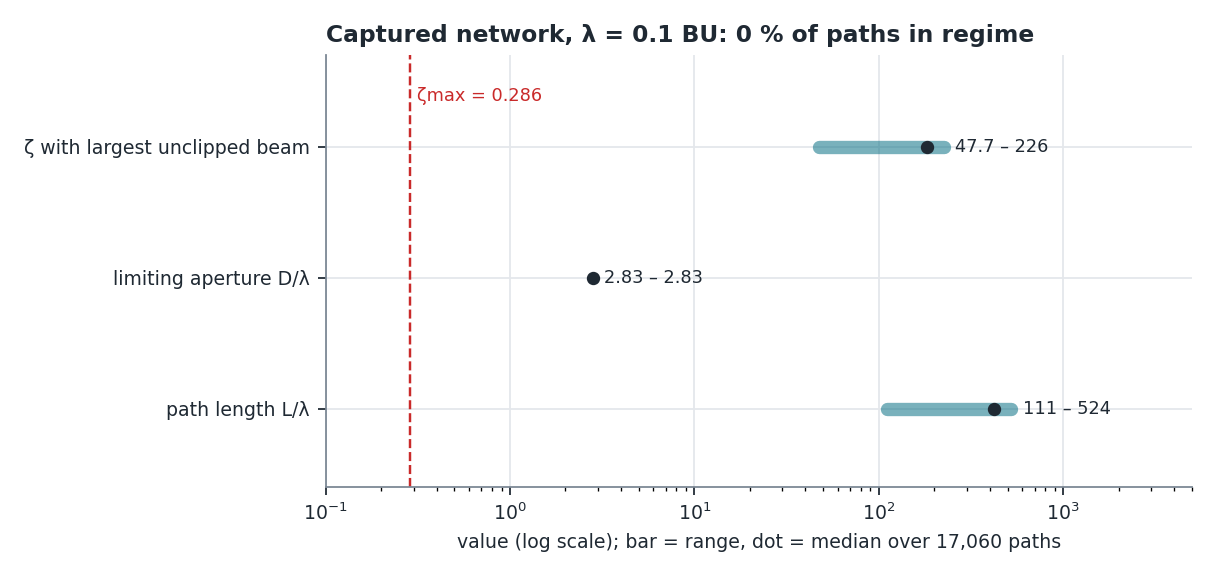
\includegraphics[width=0.64\textwidth]{figures/wave-c1-network-regime.png}
\caption{Regime map of the captured network. Bars span the range and dots mark the median over \num{17060} paths (log scale); the dashed line is the declared limit $\zeta_{\max} = 0.286$. Every path lies more than two orders of magnitude beyond it.}
\label{fig:regime}
\end{figure}

\subsection{Red-team corrections}
An independent verifier agent (a separate Claude model instance given only the artefacts and the protocol; this is adversarial review by a different agent, not human review) recomputed the MZI by its own direct plane-wave quadrature (largest difference \num{1.4e-13} over 21 phases and two ports), 16 cascade configurations (\num{1.2e-13}), the FDTD cross-check with a different window (\num{3e-15}) and the regime analysis by dynamic programming over all paths. No number was refuted. Four statements were corrected by dated notes, with the original text kept: (1) the remaining M1 residual is caused by the angular dependence of the slab coefficients, which M1 evaluates only at the central angle, not by the paraxial approximation (with an angle-independent splitter, solver and M1 differ by about \num{3e-5}); (2) the cascade scope, as described above; (3) the narrow FDTD margin; and (4) the clipping constant, rounded to 1.6449 in the protocol but computed as $\mathrm{erfc}^{-1}(10^{-3})/\sqrt{2} = 1.64526$, with no change of result.

% ===========================================================================
\section{Capacity of the captured geometry (HA-K1)}
\label{sec:capacity}

With the historical real encoding $x = (f_1,f_2,f_3,f_4,1)/\|\cdot\|$ and three decision detectors, three nested classes are compared: $\Fquad$ (argmax of arbitrary symmetric quadratic forms), $\Flin$ (argmax of $|W_k x|^2$ for an arbitrary complex $W \in \mathbb{C}^{3\times5}$; rank $\le 2$ by Proposition~\ref{prop:rank}) and $\Fgeom$ (the captured network with its 16 translations in $[-0.035, 0.035]\BU$). Thus $\Fgeom \subseteq \Flin \subseteq \Fquad$.

\paragraph{Dimensions.} Modulo the invariances of the argmax (a common additive form and a common positive scale), the local decision dimension is 12 for $\Fgeom$ at 20 random points of the box, 26 for $\Flin$ and 29 for $\Fquad$; the last two are consistent with the parameter counts $3\times9-1$ and $3\times15-15-1$. Four translations (cells \texttt{c03}, \texttt{c13}, \texttt{c23}, \texttt{c33}) have exactly zero effect on the three decision detectors: a quarter of the historically trained parameters cannot change the classifier. These values were computed while writing the protocol and are deterministic facts, not test outcomes.

\paragraph{Teacher--student test.} The preregistered test (commit \texttt{57dc002}, single execution of \SI{2292}{s} on one CPU thread) generated fresh synthetic tasks for 10 seeds, with 400 training and 2000 test inputs each, labelled by a random free linear optical map ($T_{\mathrm{lin}}$), random quadratic forms ($T_{\mathrm{quad}}$) or a random setting of the captured geometry ($T_{\mathrm{geom}}$, realisable control). Students with fixed hyperparameters were a quadratic logistic regression ($S_{\mathrm{quad}}$), a free complex linear detector classifier ($S_{\mathrm{lin}}$) and Adam on the 16 translations with the network's own gradient ($S_{\mathrm{geom}}$). Decisions used one-sided Wilcoxon signed-rank tests~\cite{wilcoxon1945} over seeds with Holm adjustment and paired bootstrap~\cite{efron1979} intervals. Every teacher and kept student geometry passed a fresh exact topology rebuild.

\begin{table}[t]
\centering
\caption{HA-K1 results over 10 seeds: mean test accuracy of each student, paired difference with 95\,\% bootstrap interval ($S_{\mathrm{lin}}-S_{\mathrm{geom}}$ for H-A1, $S_{\mathrm{quad}}-S_{\mathrm{lin}}$ for H-A2), one-sided Wilcoxon $p$ and Holm-adjusted $p$, and seeds won/tied/lost.}
\label{tab:hak1}
\footnotesize
\setlength{\tabcolsep}{4.5pt}
\begin{tabular}{@{}lccclccl@{}}
\toprule
Teacher & $S_{\mathrm{quad}}$ & $S_{\mathrm{lin}}$ & $S_{\mathrm{geom}}$ & Difference [95\,\% CI] & $p$ / Holm $p$ & W/T/L & Decision \\
\midrule
$T_{\mathrm{lin}}$ (H-A1) & 0.9752 & 0.9818 & 0.9311 & $+0.0507$ [0.0341, 0.0657] & 0.00195 / 0.00391 & 9/1/0 & supported \\
$T_{\mathrm{quad}}$ (H-A2) & 0.9779 & 0.9826 & 0.9394 & $-0.0046$ [$-0.0082$, $-0.0009$] & 0.973 / 0.973 & 3/1/6 & opposite \\
$T_{\mathrm{geom}}$ (C-A3) & 0.9868 & 0.9918 & 0.9711 & control: $S_{\mathrm{geom}} \ge 0.95$ & -- & -- & met \\
\bottomrule
\end{tabular}
\end{table}

\paragraph{Results.} Table~\ref{tab:hak1} and Figure~\ref{fig:hak1} summarise the outcome. On linear-teacher tasks the free linear student beat the captured-geometry student by $+0.051$ test accuracy, in 9 of 10 seeds with one tie: H-A1 is supported, in agreement with the dimension count. The optimizer-adequacy control was met (0.971 on realisable tasks), but the geometry student fell 0.021 short of the free linear student there, so about 0.02 of the gap reflects optimizer reach rather than representation. The second prediction \emph{failed}: on quadratic-teacher tasks the quadratic logistic student was slightly \emph{less} accurate than the linear one ($-0.005$). Since $\Flin \subseteq \Fquad$, this does not mean that the linear class represents more; with 400 training inputs and the fixed estimators, the extra quadratic capacity did not become accuracy. Majority-class rates were 0.783, 0.746 and 0.844, far below every student. The consequence is that the captured geometry is a real restriction of the linear optical class: any advantage of the approach must come from certification, robustness or cost, not from expressiveness. Activating the four inert translations is the cheapest design change suggested by this result; it has not been tested.

\begin{figure}[t]
\centering
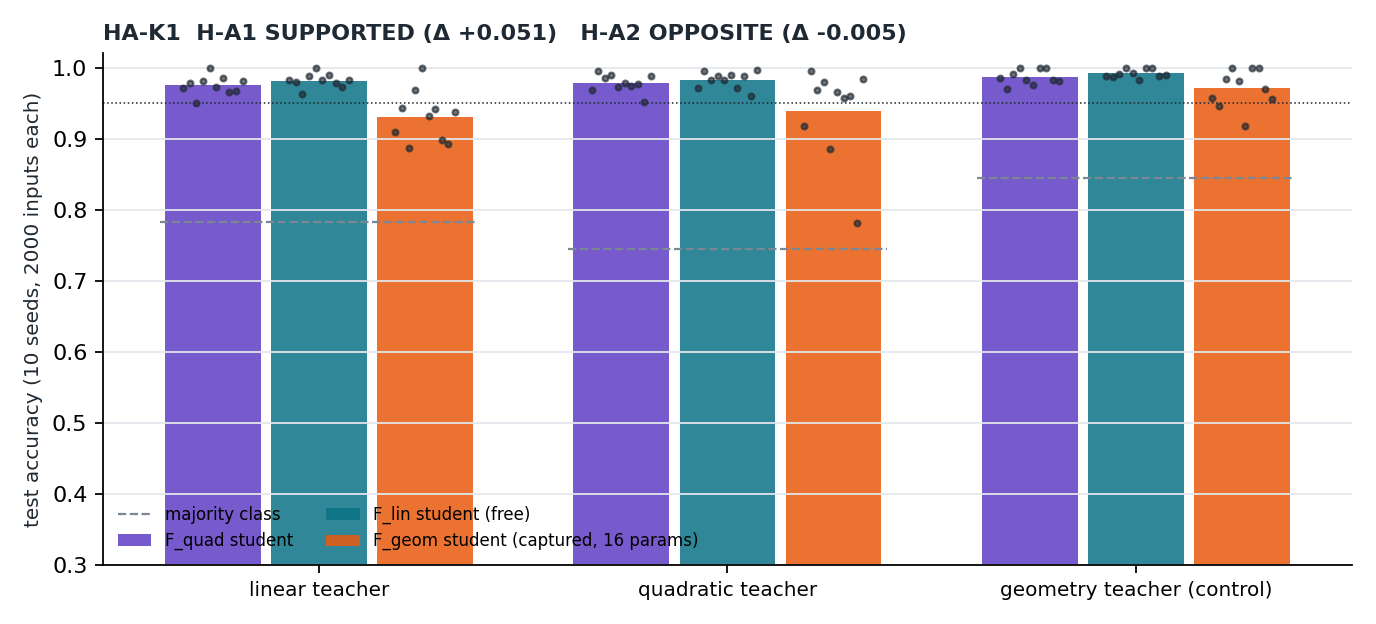
\includegraphics[width=0.78\textwidth]{figures/ha-k1-capacity.png}
\caption{HA-K1 test accuracy of the quadratic, free linear and captured-geometry students on three synthetic teacher families (bars: means over 10 seeds; dots: seeds; 2000 test inputs each). Dashed lines mark majority-class rates and the dotted line the 0.95 optimizer-adequacy threshold of the control.}
\label{fig:hak1}
\end{figure}

% ===========================================================================
\section{Compiled operator versus geometry traversal (G1)}
\label{sec:g1}

Because the represented network is linear at fixed geometry, its $8\times5$ operator $U$ and its 16 tangents $\partial U/\partial\theta_j$ can be compiled from one traversal of the five basis inputs. The compiled route reproduces the traversal to \num{6.8e-16} in fields and \num{5.4e-14} in tangents (budgets $10^{-12}$ and $10^{-9}$). The preregistered prediction (commit \texttt{b857779}) that it would be at least twice as fast when recompiled at every call was \textbf{refuted} (Table~\ref{tab:g1}): the smallest decisive ratio was 1.14. The prediction assumed that traversal cost grows with batch size inside the 133-state loop; in fact the traversal is vectorised over the batch, so both routes are dominated by the same per-state loop. Only the training step at batch 4096, where the traversal carries state $\times$ batch $\times$ 16 tangent arrays, gained a factor 16.3. With fixed geometry (inference after training, certificate replay), a cached operator is 29 to 1583 times faster on this CPU at identical outputs. Compiling $U$ with its tangents costs \SI{15.2}{ms}, the order of one traversal. Host load was not controlled, and this is a declared route inside one linear model, not a graphics, ray-tracing-core or energy result.

\begin{table}[t]
\centering
\caption{G1 timings (medians of 15 alternating repetitions, one CPU thread). Ratios are traversal time divided by compiled time.}
\label{tab:g1}
\small
\begin{tabular}{@{}lrrrrr@{}}
\toprule
Cell & Traversal & Recompiled & Cached $U$ & Ratio (recompiled) & Ratio (cached) \\
\midrule
Inference, batch 1 & 16.6\,ms & 13.9\,ms & 0.011\,ms & 1.20 & 1583 \\
Training step, batch 1 & 16.6\,ms & 16.0\,ms & 0.018\,ms & 1.04 & 912 \\
Inference, batch 150 & 15.3\,ms & 13.4\,ms & 0.019\,ms & \textbf{1.14} & 792 \\
Training step, batch 150 & 23.5\,ms & 18.6\,ms & 0.48\,ms & 1.26 & 49 \\
Inference, batch 4096 & 24.3\,ms & 15.0\,ms & 0.20\,ms & 1.63 & 122 \\
Training step, batch 4096 & 508\,ms & 31.1\,ms & 17.4\,ms & 16.3 & 29 \\
\bottomrule
\end{tabular}
\end{table}

% ===========================================================================
\section{EEG motor-imagery comparison}
\label{sec:eeg}

A separate auxiliary line evaluated simulated optical models on an 8-channel motor-imagery EEG task with 17 subjects from a competition dataset that is not redistributed here pending verification of permission. These optical models (two mesh parameterisations and an unconstrained complex matrix) are distinct from the captured Blender network. A comparison preregistered on 10 October 2026 used the same 50 external leave-one-run-out folds, the stored optical fold indices, training-only common spatial patterns and standardisation, and the same internal search budget of 36 configurations per method. The comparators were filter-bank common spatial patterns (FBCSP)~\cite{ang2008} with L2 logistic regression (H1) and EEGNet~\cite{lawhern2018} (H2).

For the primary nested estimator N1, the mean subject accuracy was \num{0.70094369} for the optical grid and \num{0.65103282} for FBCSP; the paired difference was \num{0.04991087} with bootstrap 95\,\% interval [\num{0.01479501}, \num{0.08680927}], Wilcoxon $p = \num{0.02446752}$ and Holm $p = \num{0.04893505}$ over the two-hypothesis family. This meets the original H1 rule (Figure~\ref{fig:eeg}). It does \emph{not} demonstrate superiority of a passive optical network: the optical grid includes a free digital matrix that is not a realisable unitary mesh, the grid was designed with knowledge of historical leave-one-run-out results on these subjects, and evaluation is within session on known subjects. \textbf{H2 is pending}: the EEGNet complete-fold timing pilot stopped on the 700\,MiB host-RAM floor with no timing and no H2 result, and no completed GPU H2 result was available when this manuscript was compiled.

\begin{figure}[t]
\centering
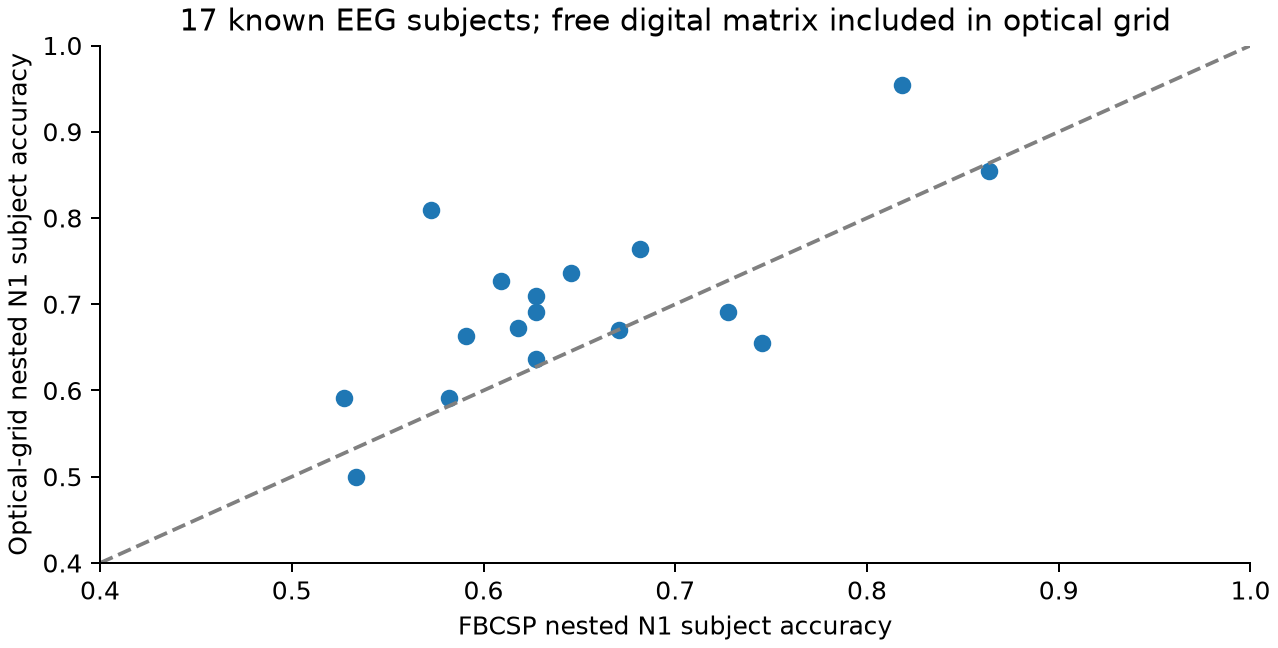
\includegraphics[width=0.56\textwidth]{figures/eeg-paired.png}
\caption{Nested primary N1 accuracy per subject: optical grid versus FBCSP (17 known subjects; dashed line: equality). The optical grid includes an unconstrained digital matrix, so the comparison does not concern a passive captured network.}
\label{fig:eeg}
\end{figure}

% ===========================================================================
\section{Discussion and limitations}
\label{sec:discussion}

\paragraph{Simulator, not device.} Everything reported here concerns a represented scalar model evaluated in software. The certificates bound observed arithmetic against that model; they say nothing about polarisation, material dispersion, detector coupling, fabrication tolerances or unobserved GPU executions, and the errors of intended versus captured geometry remain unknown. No physical optical experiment was performed.

\paragraph{The regime finding.} WAVE-C1 confirms, in one 2D geometry family and one wavelength, that free paraxial diffraction is what the no-diffraction path model misses, with an independent solver that cannot share FDTD discretisation errors. Applied to the captured scene, the same criterion shows that its ray model is far from a faithful wave description at the represented scale. This is the main constraint on any physical ambition of the approach. Physically motivated designs either build diffraction into the model, as diffractive networks do~\cite{lin2018}, or use interferometric meshes whose waveguides confine the modes~\cite{shen2017,clements2016}; a captured Blender scene would need one of these routes before any physical claim.

\paragraph{Where an advantage could come from.} HA-K1 shows that expressiveness is not the source: the geometry restricts the free linear optical class and leaves a quarter of its trained parameters inert. The Wine and EEG comparisons show no established superiority, and no end-to-end GPU cost advantage was observed. What remains is the joint certification of geometry, fields and decisions at a measured cost.

\paragraph{What would falsify the contribution.} The certificate claim is refuted by a single independently verified exact output outside its enclosure, a single invalid certified decision, or a single unbounded omitted nonzero branch. Its utility is refuted if an established differentiable-geometry stack, for example Dr.Jit~\cite{jakob2022} with interval arithmetic, delivers equivalent exact-topology and decision certificates on the same scene at lower total cost. The regime conclusion is refuted if a 3D wave simulation of a scene satisfying $\zeta \le 0.2857$ disagrees with the diffraction-inclusive path model beyond the declared budget.

\paragraph{Path to a demonstrator.} A physical test would require, in order: a rescaled geometry inside the confirmed regime (or a network model that includes the M1 diffraction factor along every path), re-run certificates for that geometry, a 3D or vector wave check, and a calibrated bench or integrated photonic implementation, possibly trained \emph{in situ}~\cite{pai2023} or with physics-aware training~\cite{wright2022}. None of these steps has been carried out.

\paragraph{Further limitations.} Iris was examined before the reported experiment; Wine uses one split with overlapping intervals; HA-K1 uses synthetic tasks and fixed student hyperparameters; G1 timings come from an uncontrolled shared host; the Lean lemmas are over the integers without Mathlib; the red team is an AI agent, not a human expert; preregistration is by public Git commits, not an external registry; and all experiments were run by the author's own tools and agents, without independent human replication.

% ===========================================================================
\section{Conclusion}
\label{sec:conclusion}

A scene editor can serve as a reproducible instrument for a coherent scalar classifier whose fields, gradients and decisions are traced to captured geometry and certified against the exact represented model, with the arithmetic core of the certificates machine-checked. The same programme of preregistered tests delimits it sharply: the represented ray model of the captured scene is outside the regime in which a path model is a faithful wave description; the geometry restricts the linear optical class it could in principle reach; no classification superiority or end-to-end GPU cost advantage was found; and a compiled operator helps only when geometry is fixed. These negatives define what a next version must change before physical claims are possible.

% ===========================================================================
\section*{Reproducibility and data availability}
\addcontentsline{toc}{section}{Reproducibility and data availability}

Code, protocols, raw results, logs and SHA256 manifests are in the public repository \url{https://github.com/Agnuxo1/Neuro3D} (MIT licence). The experiments of Sections~\ref{sec:wave}--\ref{sec:g1} and the Lean lemmas T2--T5 are on branch \texttt{claude/closure-guide-v2-20261012}: protocol commits \texttt{7327b67} (WAVE-C1), \texttt{57dc002} (HA-K1) and \texttt{b857779} (G1), each pushed before its single execution; results \texttt{0991edc} and \texttt{874a144}; red-team report \texttt{71af8e9}; Lean \texttt{ae005fa}; and the continuous-integration workflow \texttt{claude-closure-cpu.yml} (\texttt{474be60}), which reruns WAVE-C1 on Linux and compiles Lean T1--T5. Earlier evidence includes an external Linux CPU reproduction (commit \texttt{bbc06c3ace138d98873df9ba0a4d83252ebfefc8}: 27/30 held out and all 150 decisions, maximum power difference \num{3.8858e-16}), a native Linux Blender 4.5.14 run (commit \texttt{c1642ca090e8ba40bcd64f875b0d9ec39b4208ae}) and a fresh Linux interruption-and-resume test of the add-on (GitHub run 37919893102). These are automated reproductions of the author's code in other environments, not independent human replications. Every protocol states its budgets, predictions and stopping rules before execution, and failed or null attempts are archived with their logs. No external registry identifier or DOI is claimed. The Iris and Wine data are public~\cite{uciiris,uciwine}. Raw EEG recordings and derived labels and logits remain in the owner's local workspace until redistribution permission is verified; aggregate results, hashes, code and reproduction commands for legitimate data holders are public.

\section*{Use of AI tools}
Claude (Anthropic) and Codex (OpenAI) generated code, ran experiments and drafted text, including this manuscript, under the author's direction. An independent Claude verifier agent performed the red-team review of Section~\ref{sec:wave}. Decisions were routed through JEV, an advisory routing tool used by the author; its advice was recorded with provenance and is not treated as evidence. The author is responsible for the content.

\section*{Author contributions}
Francisco Angulo de Lafuente (CRediT): conceptualization, funding acquisition and resources, supervision, validation, and writing -- review \& editing.

\section*{Competing interests}
None declared.

\footnotesize
\setlength{\bibsep}{2pt plus 1pt}
\bibliographystyle{unsrtnat}
\bibliography{neuro3d_paper}

\end{document}
